% Artigo curto em formato ABNT (classe abntex2).
% Compilar: latexmk -pdf artigo.tex   (ou "make artigo" na raiz do repositório)
% Os números vêm de resultados/*.csv e resultados/resumo*.md; ao rodar as análises de novo, conferir as tabelas.
\documentclass[article,11pt,oneside,a4paper,english,brazil,sumario=tradicional]{abntex2}

\usepackage{lmodern}
\usepackage[T1]{fontenc}
\usepackage[utf8]{inputenc}
\usepackage{indentfirst}
\usepackage{graphicx}
\usepackage{microtype}
\usepackage{booktabs}
\usepackage[alf]{abntex2cite}

\graphicspath{{../graficos/}}

% PREENCHER: nomes dos integrantes, professor(a) e disciplina.
\titulo{Concentrado, mas contestado: a rivalidade no mercado brasileiro de carros 100\% elétricos (2020--2026)}
\autor{Nomes dos integrantes do grupo\thanks{Trabalho apresentado como AP2 no Ibmec. Código, dados e versão interativa: \url{https://marceufilho.github.io/carros-eletricos/}}}
\local{Brasil}
\data{Novembro de 2026}

\makeatletter
\hypersetup{
  pdftitle={\@title},
  pdfauthor={\@author},
  pdfsubject={Rivalidade setorial no mercado de carros elétricos},
  colorlinks=true,
  linkcolor=black,
  citecolor=black,
  urlcolor=blue,
  bookmarksdepth=4
}
\makeatother

\setlength{\parindent}{1.3cm}
\setlength{\parskip}{0.2cm}
\SingleSpacing

\begin{document}
\selectlanguage{brazil}
\frenchspacing

\maketitle

\begin{resumoumacoluna}
Este artigo mede a intensidade da rivalidade no mercado brasileiro de automóveis 100\% elétricos entre 2020 e outubro de 2026. Com emplacamentos por marca, importações, preços de tabela e séries macroeconômicas, todos de fontes públicas, calculamos índices de concentração e aplicamos sete métodos complementares: simulação de Monte Carlo, série temporal interrompida, painel com efeitos fixos, curva de difusão de Bass, regressão hedônica, agrupamento por k-means e \textit{gradient boosting}. O mercado cresceu de 801 para 79.415 unidades por ano entre 2020 e 2025, e o índice de Herfindahl-Hirschman passou de cerca de 1.500 para mais de 5.000 com a entrada da BYD. A liderança, porém, é contestada: a chegada do Geely EX2 está associada a uma queda de 10,1 pontos percentuais na participação da BYD ($p = 0{,}001$), enquanto nenhum dos aumentos do imposto de importação tem efeito estatisticamente distinguível de zero sobre as participações. O imposto alterou o calendário das importações, e a rivalidade se manifesta em preço e variedade: o elétrico mais barato caiu 36\% em termos reais e o número de versões à venda quase triplicou. Concluímos que o setor é altamente concentrado e intensamente disputado ao mesmo tempo, e que a ameaça à líder vem de um rival com a mesma estratégia de custo, não da política tarifária.

\vspace{\onelineskip}
\noindent
\textbf{Palavras-chave}: rivalidade setorial. veículos elétricos. concentração de mercado. estratégia competitiva. imposto de importação.
\end{resumoumacoluna}

\renewcommand{\resumoname}{Abstract}
\begin{resumoumacoluna}
\begin{otherlanguage*}{english}
This paper measures the intensity of rivalry in the Brazilian battery-electric car market from 2020 to October 2026. Using public data on registrations by brand, imports, list prices and macroeconomic series, we compute concentration indices and apply seven complementary methods: Monte Carlo simulation, interrupted time series, a fixed-effects panel, the Bass diffusion curve, hedonic regression, k-means clustering and gradient boosting. The market grew from 801 to 79,415 units a year between 2020 and 2025, and the Herfindahl-Hirschman index rose from about 1,500 to more than 5,000 after BYD entered. Leadership is nevertheless contested: the arrival of the Geely EX2 is associated with a 10.1 percentage-point drop in BYD's share ($p = 0.001$), while none of the import-tax increases has an effect on market shares that is statistically distinguishable from zero. The tax shifted the timing of imports, and rivalry shows up in price and variety: the cheapest electric car fell 36\% in real terms and the number of versions on sale almost tripled. We conclude that the sector is highly concentrated and intensely contested at the same time, and that the threat to the leader comes from a rival with the same cost strategy, not from tariff policy.

\vspace{\onelineskip}
\noindent
\textbf{Keywords}: industry rivalry. electric vehicles. market concentration. competitive strategy. import tariff.
\end{otherlanguage*}
\end{resumoumacoluna}

\textual

% ----------------------------------------------------------
\section{Introdução}

Em 2020 foram emplacados 801 automóveis 100\% elétricos no Brasil. Em 2025 foram 79.415, e só de janeiro a outubro de 2026 já são 186.514. Nesse intervalo o setor mudou de natureza: deixou de ser um nicho de importados de luxo, disputado por marcas europeias, e passou a ser um mercado de volume em que uma única marca, a BYD, vende cerca de sete em cada dez carros.

Uma participação desse tamanho sugere pouca rivalidade. Este artigo mostra que a leitura é incompleta. A pergunta que orienta o trabalho é: \textit{qual é a intensidade da rivalidade entre os concorrentes no mercado brasileiro de carros 100\% elétricos, e o que a explica?}

A resposta, em uma frase, é que o mercado é \textbf{concentrado, mas contestado}. A concentração é alta por qualquer critério usual, e ainda assim a líder perdeu participação quando um rival com a mesma estratégia de custo chegou, os preços de entrada caíram mais de um terço em termos reais e o número de modelos à venda quase triplicou. O imposto de importação, que subiu de zero a 35\% no período, mudou o calendário das importações, mas até aqui não mudou as participações de mercado.

O artigo está organizado assim: a \autoref{sec:teoria} apresenta o referencial; a \autoref{sec:metodo}, os dados e os métodos; a \autoref{sec:resultados}, os resultados em oito passos; a \autoref{sec:discussao} discute as implicações estratégicas; e a \autoref{sec:limites} registra as limitações e os próximos passos.

% ----------------------------------------------------------
\section{Referencial teórico}\label{sec:teoria}

Para \citeonline{porter1979}, a rentabilidade de um setor depende de cinco forças: a rivalidade entre os concorrentes, a ameaça de novos entrantes, a ameaça de substitutos e o poder de negociação de fornecedores e de compradores. A rivalidade tende a ser mais intensa quando os concorrentes são numerosos ou parecidos em tamanho, quando o crescimento do setor é lento, quando o produto é pouco diferenciado e quando as barreiras de saída são altas \cite{porter1980}. O mesmo autor descreve três estratégias genéricas (liderança em custo, diferenciação e enfoque) e alerta para o risco de ficar ``no meio do caminho'' entre elas.

A medida mais usada de concentração é o índice de Herfindahl-Hirschman (HHI), a soma dos quadrados das participações percentuais de cada empresa, que varia de perto de zero a 10.000. Seguindo a prática dos órgãos de defesa da concorrência, adotamos as faixas de concentração baixa (abaixo de 1.500), moderada (de 1.500 a 2.500) e alta (acima de 2.500) \cite{cade2016}. Como o HHI é uma fotografia, usamos também o índice de instabilidade de \citeonline{hymer1962}, que soma as variações absolutas de participação entre dois períodos: um mercado pode ser concentrado e, ainda assim, ter participações que mudam de mãos.

Três outros referenciais apoiam a discussão. \citeonline{mintzberg1987} distingue a estratégia como plano, manobra, padrão, posição e perspectiva, o que ajuda a ler movimentos como cortes de preço anunciados. \citeonline{chandler1962} sustenta que a estrutura segue a estratégia, o que se aplica à decisão de montar localmente. E o modelo de Uppsala \cite{johanson1977} descreve a internacionalização como um aumento gradual de comprometimento, da exportação à produção no país de destino. O lado da demanda, tratado pelo modelo de aceitação de tecnologia de \citeonline{davis1989}, fica como etapa futura (\autoref{sec:limites}).

% ----------------------------------------------------------
\section{Dados e método}\label{sec:metodo}

\subsection{Dados}

Todos os dados são públicos e agregados; a \autoref{tab:fontes} resume as fontes. A principal ressalva é que a Fenabrave só passou a publicar o ranking de elétricos por marca em 2024. Para 2020 a 2023, os totais anuais vêm da ABVE, mas a divisão entre as marcas é \textbf{estimativa do grupo}, feita a partir de rankings parciais e notícias. Tratamos essa incerteza explicitamente na \autoref{sec:montecarlo}. Além disso, o mês de outubro de 2026 é parcial (só as cinco maiores marcas, com o total estimado), e a Fenabrave divulga apenas as 15 maiores marcas de cada mês; as demais entram em ``Outros'' e ficam fora do cálculo do HHI.

\begin{table}[htb]
\caption{Fontes de dados}\label{tab:fontes}
\centering
\small
\begin{tabular}{p{5.6cm}p{5.2cm}p{3.2cm}}
\toprule
Dado & Fonte & Situação \\
\midrule
Emplacamentos mensais por marca, jan/2024 a out/2026 & \citeonline{fenabrave2026} & oficial; out/2026 parcial \\
Totais anuais, 2020 a 2023 & \citeonline{abve2024} & 2020 e 2021 a conferir \\
Divisão por marca, 2020 a 2023 & estimativa do grupo & estimado \\
Importações por país e mês & \citeonline{comexstat2026} & oficial \\
Preços zero km por modelo e mês & \citeonline{fipe2026} & oficial \\
Inflação, juros e câmbio & \citeonline{bcb2026} & oficial \\
Potência e bateria de 68 modelos & fichas técnicas & compilado; a conferir \\
\bottomrule
\end{tabular}
\fonte{Elaboração própria.}
\end{table}

\subsection{Métodos}

Os indicadores anuais são o HHI, a participação da líder (CR1) e das quatro maiores (CR4), o número de marcas com pelo menos 50 unidades e a instabilidade de Hymer-Pashigian. Sobre a série mensal de 2024 a 2026 aplicamos os métodos a seguir, cada um para responder a uma pergunta específica.

\begin{itemize}
\item \textbf{Monte Carlo.} As estimativas de 2020 a 2023 mudam a conclusão? Refizemos o HHI 5.000 vezes, perturbando cada estimativa em até 30\% e mantendo o total anual fixo.
\item \textbf{Definição de mercado.} A concentração depende do recorte? Calculamos o HHI para os elétricos, para os eletrificados (elétricos mais híbridos) e para todos os automóveis.
\item \textbf{Série temporal interrompida.} Que eventos mudaram a participação da BYD? Regressão da participação mensal sobre uma tendência e um degrau por evento, com erros-padrão robustos a heterocedasticidade e autocorrelação, complementada por um teste de quebra estrutural em data desconhecida \cite{andrews1993}.
\item \textbf{Painel com efeitos fixos.} O imposto reduz as vendas de quem só importa? Regressão do logaritmo das vendas por marca e mês sobre a alíquota a que a marca está exposta, com efeitos fixos de marca e de mês e erros agrupados por marca.
\item \textbf{Difusão de Bass.} Em que fase do ciclo está o mercado? Ajuste da curva de \citeonline{bass1969} em três cenários de mercado potencial.
\item \textbf{Regressão hedônica.} Quanto do preço se explica pelas características do carro? Regressão do logaritmo do preço sobre os logaritmos de potência e bateria e indicadores de marca chinesa e de marca premium \cite{rosen1974}.
\item \textbf{K-means.} Existem grupos estratégicos? Agrupamento dos modelos por preço, potência e bateria, com o número de grupos escolhido pelo coeficiente de silhueta.
\item \textbf{\textit{Gradient boosting}.} Que variáveis ajudam a prever as vendas de cada marca? Treino com dados até 2025 e teste em 2026.
\end{itemize}

% ----------------------------------------------------------
\section{Resultados}\label{sec:resultados}

\subsection{O mercado explodiu}

Os emplacamentos passaram de 801 unidades em 2020 para 79.415 em 2025, um crescimento médio de 151\% ao ano (\autoref{tab:anual}). Os dez primeiros meses de 2026 somam 186.514 unidades; mantido o ritmo, o ano fecharia perto de 224 mil. Na série mensal, as vendas crescem em média 5,4\% ao mês, ou seja, dobram a cada 13 meses. Para a rivalidade isso importa porque, em um mercado que dobra a cada ano, cada marca pode crescer sem tirar clientes das outras.

\begin{table}[htb]
\caption{Tamanho do mercado e concentração por ano}\label{tab:anual}
\centering
\small
\begin{tabular}{lrrlrrrr}
\toprule
Ano & Unidades & HHI & Líder & CR1 (\%) & CR4 (\%) & Marcas & Instabilidade \\
\midrule
2020 & 801 & 1.842 & Nissan & 28,7 & 79,9 & 5 & -- \\
2021 & 2.851 & 1.250 & Porsche & 18,2 & 61,4 & 10 & 48,0 \\
2022 & 8.460 & 1.516 & Volvo & 31,9 & 60,9 & 12 & 35,9 \\
2023 & 19.310 & 3.343 & BYD & 53,2 & 84,8 & 13 & 55,4 \\
2024 & 60.174 & 5.478 & BYD & 72,8 & 92,8 & 17 & 23,6 \\
2025 & 79.415 & 5.274 & BYD & 72,0 & 86,8 & 21 & 11,2 \\
2026 (jan--out) & 186.514 & 4.353 & BYD & 63,0 & 89,6 & 17 & 21,2 \\
\bottomrule
\end{tabular}
\fonte{Elaboração própria com dados de ABVE e Fenabrave. De 2020 a 2023 a divisão por marca é estimativa do grupo. Marcas: com 50 unidades ou mais. Instabilidade: índice de Hymer-Pashigian, em pontos percentuais.}
\end{table}

\subsection{De um nicho premium disputado a uma marca dominante}

Até 2022 o HHI ficou entre 1.250 e 1.842, na fronteira entre concentração baixa e moderada, e Volvo, BMW, Mercedes-Benz e Porsche somavam 51\% das vendas. A BYD entrou em 2023 com o Dolphin abaixo de R\$ 150 mil; em 2024 já tinha 72,8\% do mercado e o HHI chegou a 5.478 (\autoref{fig:hhi}). As quatro marcas premium têm hoje menos de 2\%. O índice supera o de setores brasileiros conhecidos pela concentração, como a telefonia móvel e a aviação doméstica, cujos valores de referência ficam pouco acima de 3.000.

\begin{figure}[htb]
\caption{HHI e participação das quatro maiores marcas}\label{fig:hhi}
\centering
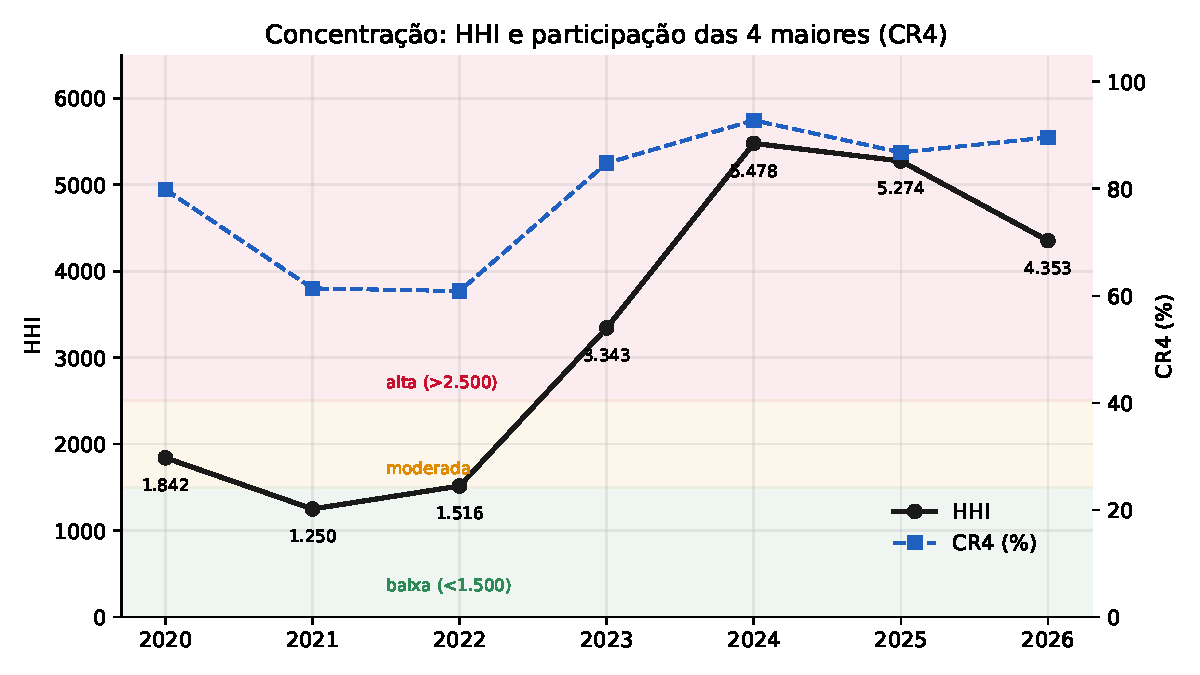
\includegraphics[width=.82\linewidth]{03_hhi_cr4.pdf}
\fonte{Elaboração própria com dados de ABVE e Fenabrave.}
\end{figure}

\subsection{A virada não depende das estimativas}\label{sec:montecarlo}

Com erro de até 30\% em cada estimativa, o HHI de 2022 fica entre 1.255 e 1.844: 47\% das simulações indicam concentração baixa e 53\%, moderada, de modo que não é possível classificar aquele ano. Em 2023, porém, o intervalo é de 3.244 a 3.457, sempre na faixa alta (\autoref{fig:mc}). A mudança de regime é um resultado robusto; os valores exatos de 2020 a 2022 não são.

\begin{figure}[htb]
\caption{HHI anual e incerteza das estimativas de 2020 a 2023}\label{fig:mc}
\centering
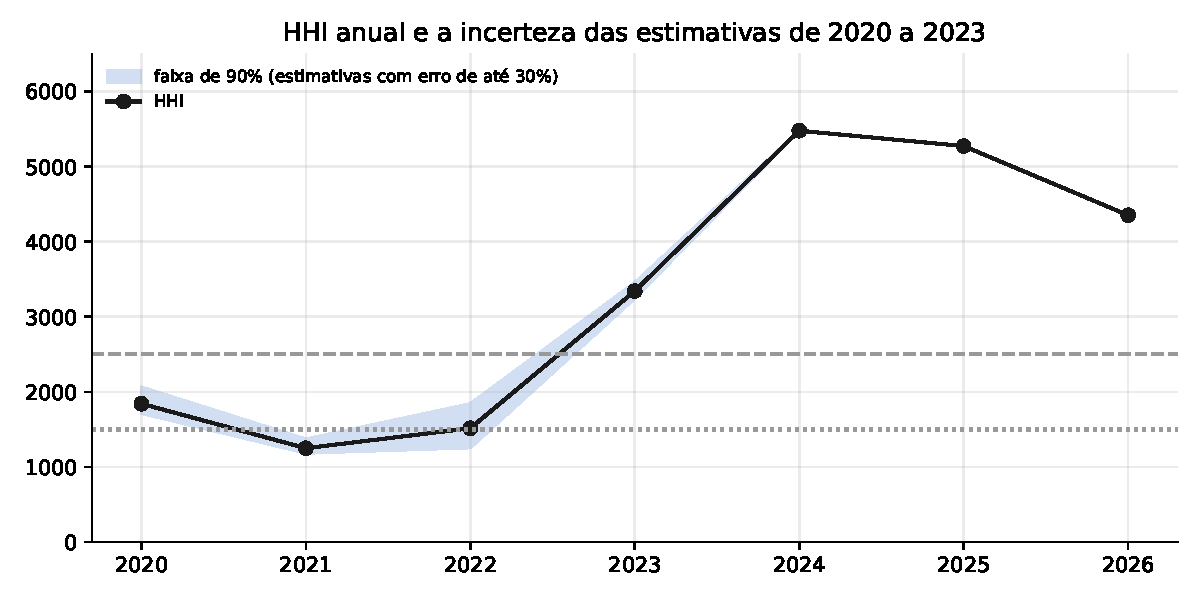
\includegraphics[width=.82\linewidth]{11_montecarlo_hhi.pdf}
\fonte{Elaboração própria. Faixa: percentis 5 e 95 de 5.000 simulações.}
\end{figure}

\subsection{A concentração depende da definição de mercado}

A \autoref{tab:definicoes} mostra o mesmo cálculo em três recortes. Entre os elétricos, a BYD tem 64\% e o HHI médio de 2026 é 4.553. Somando os híbridos, o índice cai para 2.020 (moderado), e entre todos os automóveis, para 916 (baixo), com a BYD em 9,6\%. A afirmação de que há ``quase um monopólio'' só vale no recorte mais estreito. Este artigo trata da rivalidade dentro do segmento elétrico, que representava cerca de 4\% dos automóveis emplacados no início de 2024 e cerca de 10\% em setembro de 2026.

\begin{table}[htb]
\caption{Concentração em três definições de mercado (média de 2026)}\label{tab:definicoes}
\centering
\small
\begin{tabular}{lrlr}
\toprule
Definição de mercado & HHI & Faixa & Participação da BYD (\%) \\
\midrule
Só 100\% elétricos & 4.553 & alta & 64,1 \\
Elétricos e híbridos & 2.020 & moderada & 39,7 \\
Todos os automóveis & 916 & baixa & 9,6 \\
\bottomrule
\end{tabular}
\fonte{Elaboração própria com dados da Fenabrave, janeiro a setembro de 2026.}
\end{table}

\subsection{Quem abalou a líder foi um rival, não o imposto}

A \autoref{tab:its} traz a regressão da participação mensal da BYD sobre a tendência e quatro eventos. Só um deles tem efeito estatisticamente claro: a chegada em volume do Geely EX2, em novembro de 2025, associada a uma queda de 10,1 pontos percentuais ($p = 0{,}001$). Os três degraus do imposto de importação incluídos no modelo têm coeficientes que não se distinguem de zero. O teste de quebra estrutural, que não recebe nenhuma data como informação, aponta outubro de 2025, mês de lançamento do EX2 ($F = 10{,}8$). A \autoref{fig:its} mostra a série.

\begin{table}[htb]
\caption{Série temporal interrompida: participação mensal da BYD (pontos percentuais)}\label{tab:its}
\centering
\small
\begin{tabular}{lrrr}
\toprule
Termo & Coeficiente & Erro-padrão & $p$-valor \\
\midrule
Constante & 70,90 & 2,54 & 0,000 \\
Tendência (por mês) & 0,29 & 0,23 & 0,211 \\
Imposto de 18\% (jul/2024) & 0,29 & 3,40 & 0,933 \\
Imposto de 25\% e fábrica de Camaçari (jul/2025) & $-3{,}65$ & 3,20 & 0,255 \\
Geely EX2 em volume (nov/2025) & $-10{,}15$ & 3,12 & 0,001 \\
Imposto de 35\% (jul/2026) & $-4{,}57$ & 2,88 & 0,112 \\
\bottomrule
\end{tabular}
\fonte{Elaboração própria. Mínimos quadrados com erros-padrão HAC (2 defasagens); 34 meses, de janeiro de 2024 a outubro de 2026; $R^2 = 0{,}48$.}
\end{table}

\begin{figure}[htb]
\caption{Participação mensal da BYD e eventos}\label{fig:its}
\centering
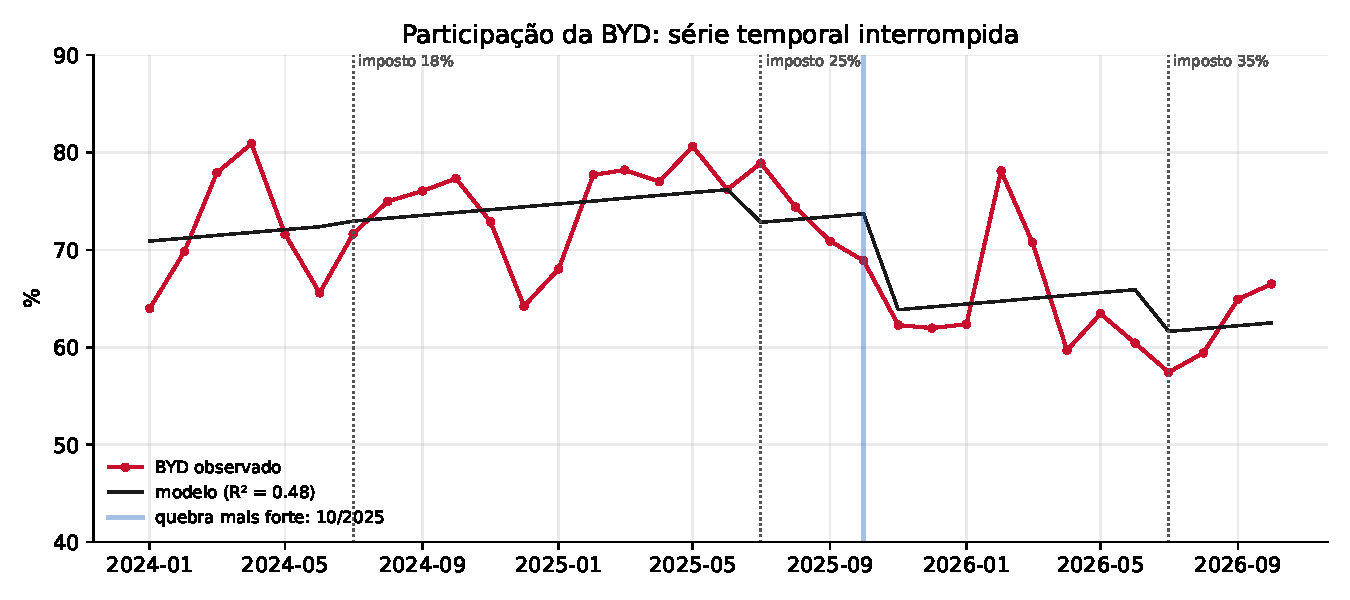
\includegraphics[width=.9\linewidth]{12_serie_interrompida_byd.pdf}
\fonte{Elaboração própria com dados da Fenabrave.}
\end{figure}

Com 34 observações e eventos próximos entre si, o sinal de cada coeficiente é mais confiável que o seu tamanho. Ainda assim, o contraste é nítido. A Geely chegou a 24,2\% do mercado em julho de 2026 e recuou para 14,1\% em setembro, o que indica que a disputa pelo segundo lugar também não está decidida.

\subsection{O imposto mudou a data das importações, não as participações}

O imposto de importação dos elétricos, zerado até 2023, subiu para 10\% em janeiro de 2024, 18\% em julho de 2024, 25\% em julho de 2025 e 35\% em julho de 2026. Como os aumentos foram anunciados com antecedência, as marcas anteciparam embarques: a média mensal de importações nos três meses anteriores a cada um dos três últimos degraus foi 7,2, 5,8 e 4,5 vezes a dos três meses seguintes (\autoref{fig:imp}). O estoque formado antes de cada alta foi vendido aos poucos com a alíquota antiga, o que adia o repasse ao preço. A China responde por 97\% das unidades importadas desde 2024, e o valor médio declarado por carro caiu de US\$ 26,6 mil em 2023 para US\$ 12,8 mil em 2026.

\begin{figure}[htb]
\caption{Importações e emplacamentos mensais de carros elétricos}\label{fig:imp}
\centering
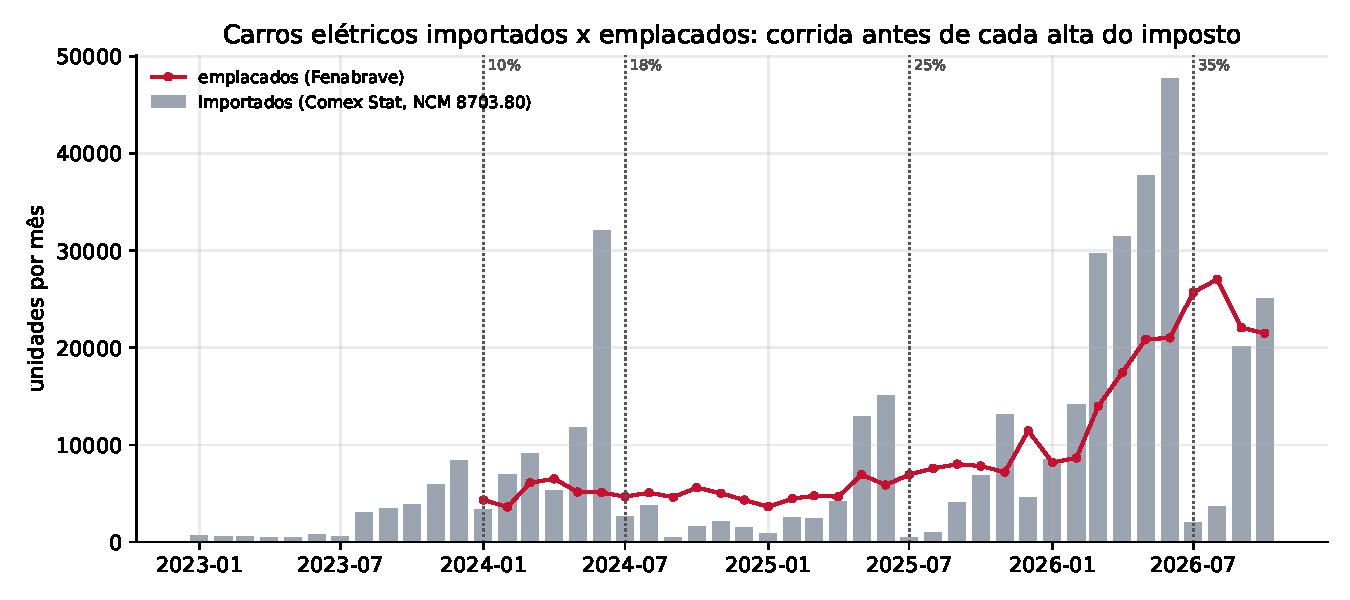
\includegraphics[width=.9\linewidth]{13_importacoes_estoque.pdf}
\fonte{Elaboração própria com dados de Comex Stat e Fenabrave.}
\end{figure}

No painel de 13 marcas e 429 observações, o coeficiente da exposição ao imposto é $-0{,}039$ (erro-padrão 0,052; $p = 0{,}453$). O sinal é o esperado, com vendas menores para quem só importa quando a alíquota sobe, mas a estimativa é imprecisa demais para sustentar qualquer afirmação. No período observado, os lançamentos de produto pesaram mais que a tarifa.

\subsection{A rivalidade aparece no preço e na variedade}

Entre janeiro de 2024 e outubro de 2026, nas 11 marcas acompanhadas mês a mês, o número de versões de elétricos zero km na tabela FIPE passou de 27 para 73, e as que custam menos de R\$ 150 mil, de nenhuma para 12. Em valores corrigidos pelo IPCA, o elétrico mais barato caiu de R\$ 157,4 mil para R\$ 100,7 mil, e o preço mediano, de R\$ 294,1 mil para R\$ 229,8 mil (\autoref{fig:precos}).

\begin{figure}[htb]
\caption{Preço real de entrada por marca e número de versões à venda}\label{fig:precos}
\centering
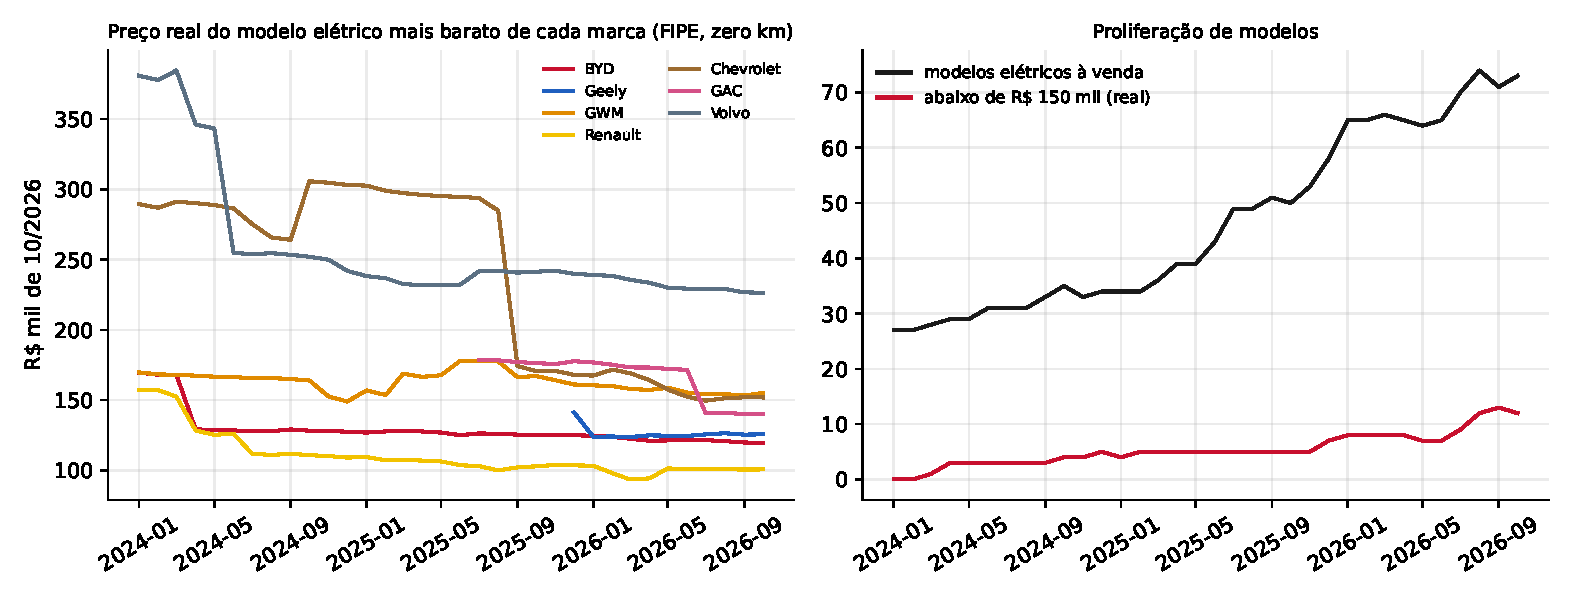
\includegraphics[width=.95\linewidth]{15_precos_fipe.pdf}
\fonte{Elaboração própria com dados da FIPE e do Banco Central.}
\end{figure}

A regressão hedônica (\autoref{tab:hedonica}) mostra que, com a mesma potência e a mesma bateria, um modelo de marca chinesa custa 26\% menos e um de marca premium, 24\% mais que os demais. É a liderança em custo de \citeonline{porter1980} em números. O agrupamento por k-means encontrou três grupos estratégicos (silhueta de 0,47): um de entrada, com 8 modelos e preço mediano de R\$ 125 mil; um intermediário, com 34 modelos e R\$ 232 mil; e um de topo, com 26 modelos e R\$ 543 mil. As marcas chinesas são 62\% e 59\% dos dois primeiros grupos e 27\% do terceiro, onde enfrentam as marcas tradicionais.

\begin{table}[htb]
\caption{Regressão hedônica do logaritmo do preço}\label{tab:hedonica}
\centering
\small
\begin{tabular}{lrrr}
\toprule
Termo & Coeficiente & Erro-padrão & $p$-valor \\
\midrule
Constante & 7,399 & 0,414 & 0,000 \\
Logaritmo da bateria (kWh) & 0,785 & 0,217 & 0,000 \\
Logaritmo da potência (cv) & 0,365 & 0,140 & 0,009 \\
Marca chinesa & $-0{,}302$ & 0,060 & 0,000 \\
Marca premium & 0,218 & 0,070 & 0,002 \\
\bottomrule
\end{tabular}
\fonte{Elaboração própria. Mínimos quadrados com erros-padrão robustos (HC1); 68 modelos; $R^2 = 0{,}87$. Preços da FIPE em outubro de 2026.}
\end{table}

\subsection{Para onde vai o mercado, e o que não se pode saber}

O ajuste da curva de Bass indica que a adoção ocorre por imitação: o coeficiente de imitação fica entre 0,076 e 0,083 ao mês, e o de inovação é praticamente zero. O teto do mercado, porém, não pode ser estimado enquanto a curva só acelera. Fixando o potencial em 2, 5 ou 10 milhões de carros, o ajuste é praticamente o mesmo ($R^2$ de 0,78, 0,81 e 0,81), mas o pico de vendas viria em junho de 2028, setembro de 2029 ou julho de 2030, com 41 mil, 97 mil ou 190 mil carros por mês (\autoref{fig:bass}). São cenários, não previsões.

\begin{figure}[htb]
\caption{Difusão de Bass em três cenários de mercado potencial}\label{fig:bass}
\centering
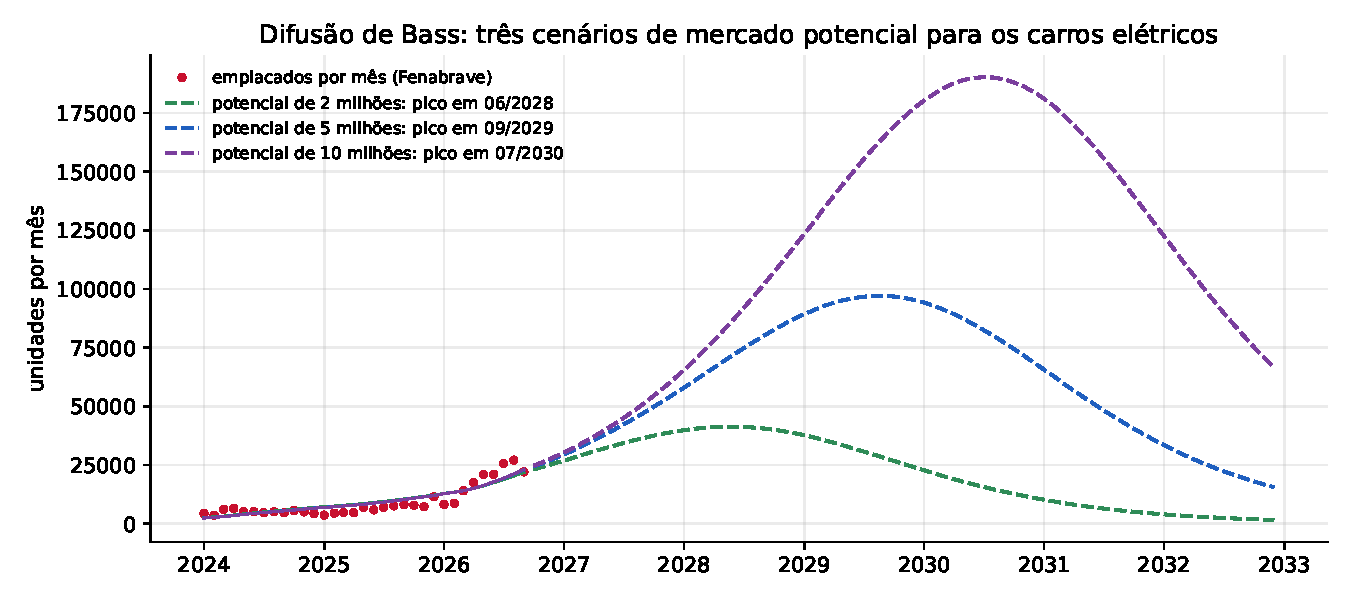
\includegraphics[width=.9\linewidth]{14_bass_difusao.pdf}
\fonte{Elaboração própria com dados da Fenabrave.}
\end{figure}

O exercício de previsão confirma a cautela. O modelo de \textit{gradient boosting} prevê as vendas mensais de cada marca em 2026 com $R^2$ de 0,82 fora da amostra, contra 0,80 da regra de repetir o mês anterior. Sem a venda defasada, o $R^2$ cai para 0,14, e as variáveis que mais pesam são o número de modelos elétricos da marca e o seu preço de entrada. Com 207 observações de treino e 81 de teste, o exercício serve para ordenar fatores, não para prever.

% ----------------------------------------------------------
\section{Discussão estratégica}\label{sec:discussao}

Os resultados permitem reavaliar a força ``rivalidade'' de \citeonline{porter1979} no setor. Há dois fatores que a atenuam: o crescimento muito rápido, que permite a todos vender mais, e a concentração elevada. E há três que a intensificam: produtos cada vez mais parecidos na faixa de entrada, concorrentes com a mesma estratégia genérica e compradores com mais opções a cada mês. O saldo, na avaliação do grupo, é de rivalidade em alta, mesmo com o HHI acima de 4.000.

\textbf{Estratégias genéricas.} As marcas chinesas venceram pela liderança em custo, apoiada na verticalização da bateria e na escala global. As marcas premium europeias mantiveram a diferenciação, mas em um nicho que encolheu de mais da metade do mercado para cerca de 2\%. A disputa relevante passou a ser entre empresas com a mesma estratégia, que é a situação em que \citeonline{porter1980} espera competição por preço.

\textbf{Barreiras à entrada e internacionalização.} A sequência seguida pelas líderes (importar, formar rede, montar em regime de kits e depois produzir localmente) reproduz o comprometimento gradual descrito por \citeonline{johanson1977}, e a decisão de montar no país é um caso de estrutura que segue a estratégia \cite{chandler1962}. Com a alíquota em 35\%, a produção local deixa de ser opção e passa a ser condição para competir em preço. O efeito ainda não aparece nas participações, mas a barreira para um entrante que apenas importe é hoje muito maior que em 2023.

\textbf{O que esperar.} Enquanto o mercado dobrar a cada ano, a guerra de preços é sustentável, porque o volume compensa a margem. Quando o crescimento desacelerar, o que a curva de Bass indica que acontecerá em algum momento entre 2028 e 2030, a mesma disputa tende a se tornar destrutiva, com saída ou consolidação das marcas menores. Para as marcas premium, o caminho coerente é o enfoque: defender um nicho de alto valor em vez de disputar volume.

% ----------------------------------------------------------
\section{Limitações e próximos passos}\label{sec:limites}

As principais limitações são quatro. Primeiro, a divisão por marca de 2020 a 2023 é estimada; a simulação mostra que a conclusão central não depende dela, mas os valores anuais desse período são aproximados. Segundo, a série mensal oficial tem 33 meses completos, o que basta para identificar a direção dos efeitos, não o seu tamanho. Terceiro, potência, bateria e as datas de início de montagem local foram compiladas pelo grupo e precisam de conferência. Quarto, o código de importação usado (NCM 8703.80.00) inclui veículos elétricos pequenos que não são emplacados como automóveis, de modo que importações e emplacamentos não fecham entre si.

Falta também o lado do consumidor. O grupo preparou um questionário com dez itens em escala Likert, baseado no modelo de aceitação de tecnologia de \citeonline{davis1989}, que mede utilidade percebida, facilidade de uso percebida, atitude e intenção de compra de um carro elétrico. A aplicação na turma e a estimação do modelo são o próximo passo; este artigo não traz resultados dessa etapa.

\section{Conclusão}

O mercado brasileiro de carros 100\% elétricos é altamente concentrado e intensamente disputado ao mesmo tempo. A concentração nasceu de uma vitória por custo, e a ameaça à líder vem de outra marca com a mesma estratégia. A política tarifária, até aqui, alterou quando os carros chegam ao país, não quem os vende. A rivalidade se expressa menos nas participações de mercado e mais no que o consumidor paga e no que pode escolher: preços de entrada um terço menores e quase três vezes mais modelos em menos de três anos.

\postextual
\bibliography{referencias}

\end{document}
